Since no mirror specification was available for our super mirrors, we decided to obtain our own experimentally, see figure \ref{fig:trans_mirrors}. We expected, at optimal wavelength \SI{852}{\nano\meter}, to get very tiny transmissions on order tens of part per million (ppm). Therefore normal means did not work, i.e. just measuring power before and after the mirror with a power meter. To obtain the data we used the tunable Ti:Sapph laser, the output of which was sent through an AOD connected to the TTL switch board, such that the light was fully amplitude modulated at an arbitrary frequency. A detector was placed after the mirror and its output was sent to a lock-in amplifier and demodulated at the given amplitude modulation frequency. The resulting mirror transmissions as function of wavelength are shown in figure \ref{fig:trans_mirrors}.

\begin{figure}[H]
\centering
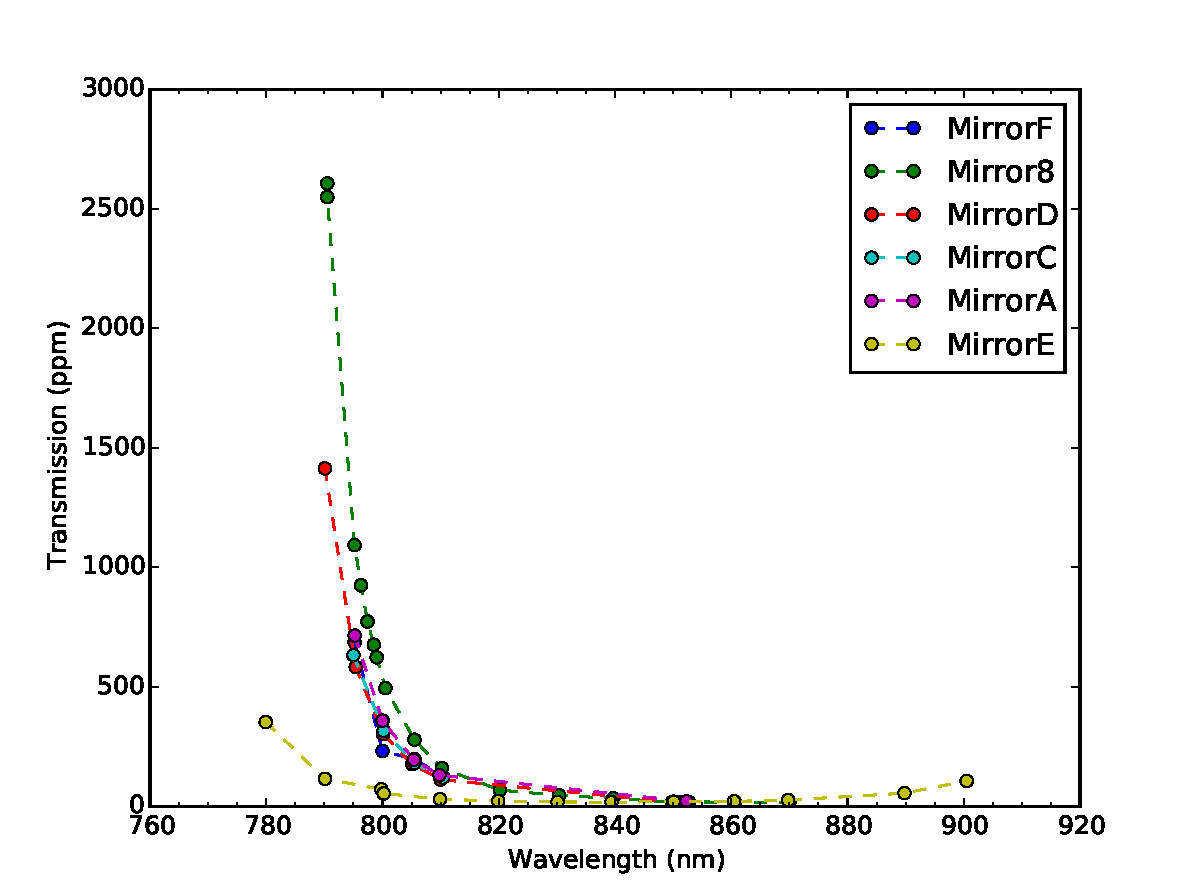
\includegraphics[scale=0.7]{mirror_transmissions.pdf}
\caption{Transmission as a function of wavelength for our super polished mirrors. They all have the same transmission curve except from the ``special" mirror 8, which has a curve shifted of the rest. Mirrors denoted with a letter are curved and mirrors with a number are flat.}
\label{fig:trans_mirrors}
\end{figure}

Simultaneously we were testing mirrors with different coatings, to find a curved mirror with a higher transmission than the flat bottom mirror, in order to utilize a different cavity coupling regime instead of a critical coupled one, see section \ref{sec:opt_cav}. Whereas critical coupling is good for cooling, different experiments, such as squeezing, call for an alternative coupling regime. By coincidence we found that one of our already in stock super mirrors had a slightly shifted transmission curve, clearly deviating from the rest of the mirrors from the same coating run. Mirror 8 combined with mirror E has the most shifted apart transmission curves, but still fulfill critical coupling with each mirror presenting \SI{20}{ppm} at \SI{852}{\nano\meter} see figure \ref{fig:trans_e_8}.


\begin{figure}[H]
\centering
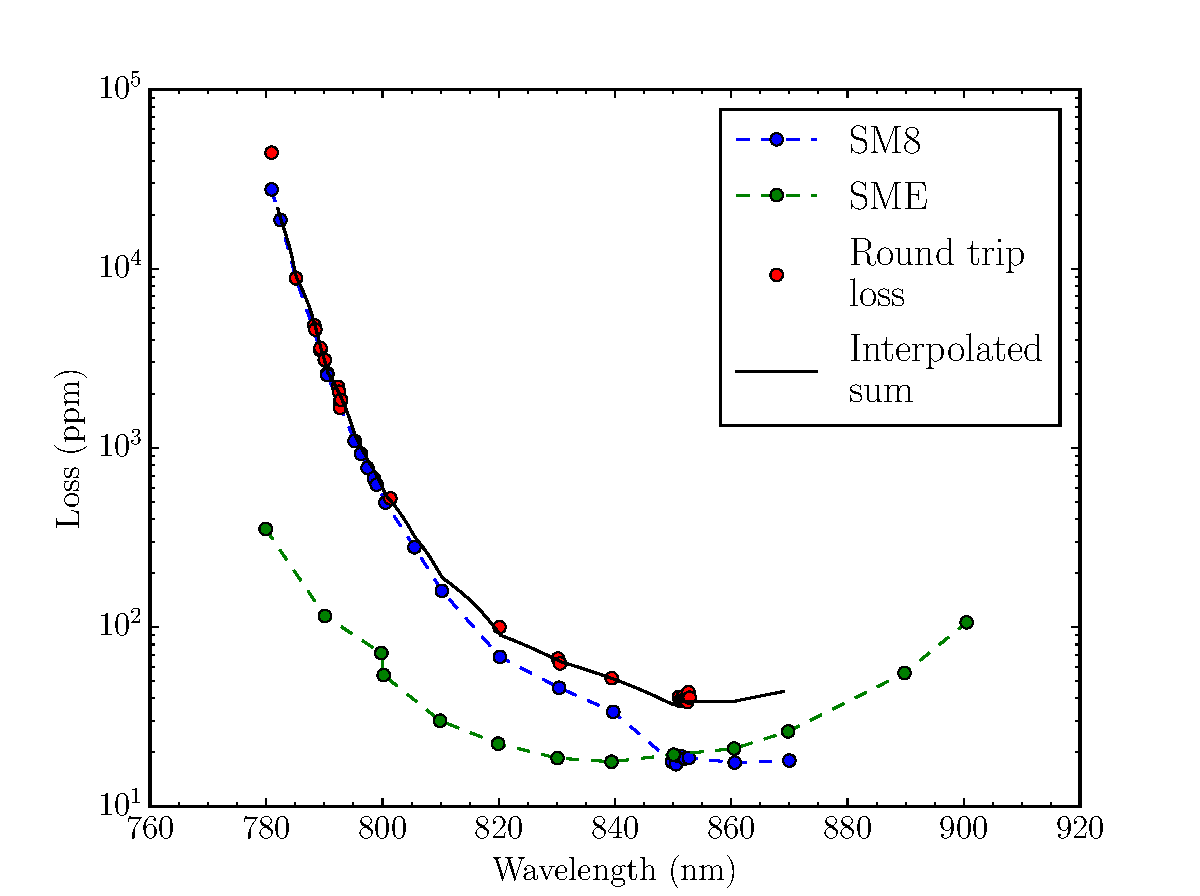
\includegraphics[scale=0.7]{mirror_e_8.pdf}
\caption{Mirror transmission presented on a log scale for mirrors 8 (green) and E (blue). An interpolated sum (black) of the two mirror transmissions together with an actual measured round trip loss (red) for an assembled bare cavity shows that these two mirrors have very little loss, when combined into a cavity.}
\label{fig:trans_e_8}
\end{figure}

By tuning our wavelength up or down in wavelength, we can choose how deep into the different cavity coupling regimes we can be. This is truly a neat feature of our cavity.